\subsection{Medidas de distancia de texto}
\subsubsection{Conceptos básicos}
\paragraph{Information retrieval}
Information retrieval (IR) se define como encontrar material (generalmente documentos) de una naturaleza desestructurada (generalmente texto) que satisfaga una necesidad de información de grandes colecciones (generalmente almacenadas en computadoras) \citep{schutze2008introduction}.

\bigskip El IR utiliza técnicas probabilísticas, pero también, en los últimos años, investigadores se han centrado en técnicas basadas en conocimiento. Estas últimas, han hecho una significante contribución al IR “inteligente”. Más recientemente, la investigación se ha volcado a nuevas técnicas de aprendizaje inductivo basadas en \textit{inteligencia artificial} (IA), las cuales incluyen redes neuronales, aprendizaje simbólico y algoritmos genéticos \citep{chen1995machine}. Cuando hablamos de aprendizaje, nos referimos a un fenómeno multifacético. Los procesos de aprendizaje incluyen la adquisición de un nuevo conocimiento declarativo, la organización del nuevo conocimiento, representaciones efectivas y un descubrimiento de nuevos hechos y teorías a través de la observación y la experimentación. Desde el nacimiento de la era de las computadoras, estas capacidades han querido ser implantadas en las mismas. El estudio y el modelado en computadoras del proceso de aprendizaje en múltiples manifestaciones constituye el propósito principal del \textit{Machine Learning} (ML) \citep{mitchell2013artificial}.

\bigskip Los Sistemas de Recomendación a los cuales se hace foco en este trabajo, aplican técnicas que no son más que conceptos derivados del IR y algunos del ML. Técnicas probabilísticas y determinísticas son utilizadas para extraer información relevante desde diferentes orígenes de datos, así como también generar información valiosa a partir de ellos. Para este último propósito, se han desarrollado métodos basados en el aprendizaje inductivo que demostraron ser muy efectivos y, en algunos casos, tener modelos simples y aplicables que permiten desarrollar RS eficaces y escalables.

\paragraph{Unidad de documento}
Una \textit{unidad de documento}, es una secuencia de caracteres de longitud fija con las cuales se va a trabajar. Estas secuencias de caracteres pueden estar codificadas por uno o varios bytes o esquemas de codificación multibyte, como UTF-8 o varios estándares específicos de algún país o compañía. Una vez que la codificación esté determinada, se debe decodificar la secuencia de bytes a una secuencia de caracteres.

\paragraph{Stopwords}
En informática, se llama stopword a palabras que se filtran antes o después del procesamiento de datos del lenguaje natural \citep{leskovec2014mining}. Generalmente, este tipo de palabras son extremadamente comunes, y podrían tener poco valor en el momento de seleccionar documentos que coincidan con las necesidades de un usuario \citep{schutze2008introduction}.

\bigskip Entonces es necesario seleccionar una lista de stopwords, que serán filtradas en el procesamiento de las unidades de documento, estas listas son llamadas \textit{stop lists}. La estrategia general para el armado de stop lists, es ordenar los términos por \textit{collection frequency}, es decir, el número total de veces que aparece un término en la colección de documentos. Una vez hecho esto, es necesario tomar los términos más frecuentes, a veces filtrados a manos según su contenido semántico relativo al dominio de los documentos que están siendo indexados.

\paragraph{Tokenización}
Dado una secuencia de caracteres y una unidad de documento definida, la \textit{tokenización} es la tarea de dividirla en distintas piezas, llamadas \textit{tokens}, y, quizás en el mismo momento, desechar ciertos caracteres (como signos de puntuación). Un ejemplo de tokenización de una secuencia de caracteres en idioma inglés, podría ser:

\begin{verbatim}
Input: Friends, Romans, Countrymen, lend me your ears;
Output: [Friends] [Romans] [Countrymen] [lend] [me] [your] [ears]
\end{verbatim}

Estos tokens, son frecuentemente confundidos con palabras, pero es importante hacer la distinción entre token y tipo. Un token es una instancia de una secuencia de caracteres en un documento en particular que están agrupados juntos como una unidad semántica útil para procesamiento. Un \textit{tipo} es la clase de todos los tokens que contienen la misma secuencia de caracteres. Un \textit{término} es un tipo, que es incluido en un diccionario de un sistema de IR. Por ejemplo, si un documento a ser indexado es “to sleep perchance to dream”, existen 5 tokens, pero solo 4 tipos (ya que hay dos instancias del token “to”). Sin embargo, si “to” es desechada por ser un stopword, habrá entonces 3 términos: “sleep”, “perchance” y “dream”.

\paragraph{Similaridad}\label{paragraph:similaridad}
Es de interés poder cuantificar la relación entre los objetos de texto. Existen distintas maneras de medir esa relación. En general se habla de medidas de proximidad \citep{xu2008clustering}. Las medidas de proximidad son una generalización para las medidas de similaridad y disimilaridad. En este trabajo utilizaremos medidas de similaridad comúnmente encontradas en la literatura \citep{resnik1995using, lin1998information, gomaa2013survey, harispe2015semantic}. Debido al propósito de este trabajo, es de interés, en particular, la similaridad semántica en taxonomías \citep{resnik1995using}, que se basa en el contenido de información de las unidades documentales.

\bigskip Las medidas basadas en contenido de información de una unidad de documento (o concepto) en una taxonomía, utilizan el siguiente enfoque. Se define \(p(t)\) como:
\[p(t)=\frac{cantidad\>de\>palabras\>asociadas\>a\>una\>definici\acute{o}n\>\>sus\>hijos}{cantidad\>total\>de\>palabras\>en\>el\>corpus}\]

De esta forma, el nodo raíz tendrá \(p(t) =0\), mientras los nodos hojas, tendrán valores cercanos a 1. Se define el contenido de información \(I(t) =0\) como:
\[I(t)=-\log p(t)\]

Aplicando el logaritmo negativo a \(p(t) =0\) se logra que los nodos hoja, siendo conceptos muy específicos, contengan mucha información, y que los nodos más genéricos que se encuentran cerca de la raíz contengan un contenido de información que, por lo contrario, tienda a cero.

\bigskip \cite{resnik1995using} define, en un conjunto de conceptos \(C\) en una taxonomía \textit{es-un}, que permite herencia múltiple, que la similaridad entre dos conceptos es la medida en que ellos comparten información en común, indicado, en este tipo de taxonomías, por el nodo inmediato de más alto nivel que los subsume a ambos, el \textit{subsumidor mínimo} (minimum subsumer o ms por sus siglas en inglés).

\bigskip Considerando dos términos \(t_i\) y \(t_j\), y a \(S(t_i, t_j\)) al conjunto de ancestros comunes de \(t_i\) y \(t_j\), se define al subsumidor mínimo, \(ms(t_i, t_j)\), como al término de \(S(t_i, t_j)\) que contiene el máximo contenido de información:
\[\max_{t \in s(t_i,t_j)} I(t) = I(ms(t_i,t_j))\]

La medida de similaridad de \cite{resnik1995using} \(S_R\), es entonces, el contenido de información del subsumidor mínimo de dos términos:
\[S_R = I(ms(t_i,t_j))\]

\bigskip El enfoque anterior, posee la siguiente particularidad: no tiene en cuenta la similaridad de los nodos con respecto a su subsumidor mínimo. Es intuitivo pensar que dos conceptos abstractos (nodos ubicados en posiciones más cercanas al subsumidor mínimo) son más parecidos entre sí que dos conceptos específicos (más alejados del subsumidor mínimo) \citep{lin1998information}. Para solucionar esto, \cite{lin1998information} tiene en cuenta dos aspectos para calcular la similaridad entre dos conceptos en este tipo de taxonomías: \begin{enumerate*} [label=(\roman*)] \item La cantidad de información; y \item La ubicación relativa entre los nodos hijos respecto al subsumidor mínimo. Definida como la similaridad de \cite{resnik1995using}. \end{enumerate*}

\bigskip La medida de Lin es:
\[S_L(t_i, t_j)=\frac{2S_R(t_i,t_j)}{I(t_i)+I(t_j)}\]

El resultado de esta medida, estará normalizada en el rango \([0, 1]\) y obtiene que nodos más generales, con menor cantidad de información, son más similares entre sí, que dos nodos específicos (ya que la cantidad de información de los mismos aumentará el denominador de la ecuación) para el mismo subsumidor mínimo. Se ha demostrado que esta definición de similaridad produce una correlación ligeramente mayor con los juicios humanos.

\paragraph{Medidas de proximidad}
Proximidad es la generalización de similaridad y disimilaridad. La función disimilaridad, también conocida como función de distancia, en un conjunto de datos X, es definida para satisfacer las condiciones. Las condiciones mencionadas, son las utilizadas por \cite{xu2008clustering} y de relevancia en el presente trabajo:

\begin{enumerate}
	\item Simetría,
	\[D(x_i,x_j)=D(x_j,x_i);\]

	\item Positividad,
	\[D(x_i,x_j) \geq 0 \quad \forall x_i,x_j;\]
\end{enumerate}

De forma, análoga la función de similaridad es definida satisfaciendo las condiciones:
\begin{enumerate}
	\item Simetría,
	\[S(x_i,x_j)=S(x_j,x_i);\]

	\item Positividad,
	\[0 \leq S(x_i,x_j) \leq 1, \quad \forall x_i,x_j\]
\end{enumerate}

Si bien el término matemático de distancia exige una serie de supuestos rigurosos \citep{xu2008clustering}, en este trabajo utilizaremos la noción de distancia y de disimilaridad en forma indistinta, y nos basaremos en las medidas de proximidad habitualmente utilizadas para comparación de texto. Por lo tanto, Para transformar una medida de similaridad \(S(x_i,x_j)\) en una de distancia \(D(xi,xj)\) que cumpla \(0 \leq D(x_i,x_j) \leq 1\), haremos la normalización de la misma en el intervalo \([0,1]\) y luego aplicaremos el cálculo \(D(x_i,x_j) = 1 - S(x_i,x_j)\) y recíprocamente \citep{leale2013novel}.

\paragraph{Modelo de espacio vectorial}
En el modelo de espacio vectorial, un texto es representado como un vector de términos. Si las palabras son elegidas como términos, entonces cada palabra del vocabulario sería una dimensión independiente en el espacio vectorial \citep{singhal2001modern}. Todo texto puede ser representado por un vector en este espacio dimensional. Si un término pertenece a un documento, éste obtiene un valor distinto de cero en el vector, junto con la dimensión correspondiente al término. Como un documento contiene un conjunto limitado de términos (el vocabulario puede contener millones de términos), muchos de los vectores pueden ser muy dispersos. La mayoría de los sistemas basados en vectores trabajan en el cuadrante positivo, es decir, a ningún término se le asigna un valor positivo.

\bigskip Para asignar un valor numérico a un documento en una consulta, el modelo mide la similaridad entre el vector ingresado en ella y el vector del documento al cual se quiere consultar. La similaridad entre dos vectores no es inherente al modelo. Típicamente, el ángulo entre los dos vectores es usado como medida de divergencia entre los mismos, y el coseno del ángulo es usado como similaridad numérica, ya que el coseno tiene la propiedad de ser tener resultado 1 cuando los vectores son idénticos y 0 cuando los vectores son ortogonales (explicado en detalle más adelante). Como una alternativa, el producto escalar entre dos vectores, es también usado como medida de similaridad. Si todos los vectores están forzados a tener longitud 1, es decir, vectores unitarios, entonces el coseno del ángulo entre los vectores, tiene el mismo resultado que el producto escalar.

\bigskip Si \(\overrightarrow{D}\) es el vector del documento y \(\overrightarrow{Q}\) es el vector de la consulta, la similaridad entre \(\overrightarrow{D}\) y \(\overrightarrow{Q}\) es representada como:
\[S(\vec{D},\vec{Q})=\sum_{ti \in Q,D}^{ }{W_{t_{iQ}}.W_{t_{iD}}}\]

donde \(W_{t_{i \overrightarrow{Q}}}\) es el valor de la componente número \(i\) del vector \(\overrightarrow{Q}\) y \(W_{t_{i \overrightarrow{D}}}\) es el valor de la componente número \(i\) del vector \(\overrightarrow{D}\). También definido como el peso del término \(i\) en el documento \(D\). Cualquier término no presente en la consulta o en el documento tendrá valor cero en \(W_{t_{i \overrightarrow{Q}}}\) o \(W_{t_{i \overrightarrow{D}}}\), por lo cual es posible hacer la sumatoria solo de los términos en común entre la consulta y el documento.

\paragraph{Distancia del coseno}
La distancia del coseno puede ser la mayor frecuentemente aplicada en términos de similaridad en IR \citep{korenius2007principal}. Al aplicar la distancia del coseno se obtiene un resultado que se encuentra en el rango \([-1, 1]\). El valor \(-1\) significa que los vectores tienen la misma dirección, pero sentidos opuestos. El valor \(1\), por lo contrario, significa que el ángulo comprendido entre los vectores es cero.

\bigskip Particularmente en IR, es de interés el intervalo \([0, 1]\) ya que todos los componentes de un vector que representa a un documento, son no negativos. De esta interpretación, se deriva la definición de la distancia del coseno restando la medida del coseno, de su máximo valor:
\[d_c(\vec{D}_i, \vec{D}_j) = 1 - cos(\vec{D}_i, \vec{D}_j) = 1 - \frac{{\vec{D}_i}'\vec{D}_j}{\sqrt{{\vec{D}_i}'\vec{D}_i}\sqrt{{\vec{D}_j}'\vec{D}_j}}\]

donde \(i \leq i,j \leq n\). Los símbolos \(\overrightarrow{D_i}\) y \(\overrightarrow{D_j}\) son documentos en forma de vectores y dces la distancia entre ellos.

\bigskip Para simplificar, y teniendo en cuenta que estamos hablando de documentos en forma de vectores, la distancia del coseno se puede derivar de la fórmula del \textit{producto escalar} (producto punto). Siendo \(\overrightarrow{D_i}\) y \(\overrightarrow{D_j}\) dos documentos en forma de vectores, se define el producto escalar entre ellos, como:
\[\vec{D}_i.\vec{D}_j = \left \| \vec{D}_i \right \|.\left \| \vec{D}_j \right \|.cos(\theta)\]

siendo \(\left \|\overrightarrow{D_i}\right \|\) y \(\left \|\overrightarrow{D_j}\right \|\) los módulos de los vectores \(\overrightarrow{D_i}\) y \(\overrightarrow{D_j}\) respectivamente, y $\theta$ el ángulo formado entre ellos. Entonces:
\[cos(\theta) = \frac{\vec{D}_i.\vec{D}_j}{\left \| \vec{D}_i \right \|.\left \| \vec{D}_j \right \|}=\frac{\sum_{i=1}^{n}{{d_i}_i{d_j}_i}}{\sqrt{\sum_{i=1}^{n}{{d_i}_i^{2}}}\sqrt{\sum_{i=1}^{n}{{d_j}_i^{2}}}}\]

Donde \(d_i\) y \(d_j\) son los componentes de los vectores \(\overrightarrow{D_i}\) y \(\overrightarrow{D_j}\) respectivamente.

\subsubsection{Term Frequency}
También conocido en la literatura como \textit{Bag of words} (bolsa de palabras), \textit{Term Frequency}, o TF; es una técnica donde el orden exacto de los términos es ignorado, pero se basa en número de ocurrencia de cada uno de ellos \citep{christopher2008introduction}.

\bigskip Si comparamos las frases en inglés \textit{“Mary is quicker than John”} y \textit{“John is quicker than Mary”}, desde esta perspectiva, son idénticas. Esto conlleva a ciertos problemas desde el punto de vista semántico, ya que, si bien el número de ocurrencia de términos es el mismo, el significado de las frases es opuesto. Las palabras son contadas en una \textit{bolsa}, lo cual difiere de la definición matemática de \textit{conjunto}, que no considera los elementos repetidos. Cada palabra corresponde a una dimensión en el espacio de datos resultante y cada documento corresponde a un vector compuesto por valores no negativos en cada dimensión \citep{huang2008similarity}. Con los documentos representados como vectores, se mide el grado de similaridad de dos documentos como la correlación entre los vectores correspondientes, que puede ser cuantificada como el coseno del ángulo entre ellos. Entonces, es posible obtener la distancia entre dos documentos en forma de vectores \(\overrightarrow{D_1}\) y \(\overrightarrow{D_2}\) aplicando:
\[d(\vec{D}_1, \vec{D}_2) = 1 - \frac{\vec{D}_1 \vec{D}_2}{\left \| \vec{D}_1 \right\| \left \| \vec{D}_2 \right\|}\]

Hasta ahora, no se ha mencionado que implicancia tiene la frecuencia de cada término en un documento, en el momento de realizar la consulta: un documento que menciona un término más frecuentemente tiene más similitud con la query en cuestión, por lo tanto, recibirá una valoración mayor. Lo anterior, significa que se asigna un peso a cada término, en una relación directamente proporcional al número de ocurrencias del mismo en el documento \citep{christopher2008introduction}.

\subsubsection{Term Frequency/Inverse Document Frequency}
La valoración de un término, no tiene una relación directamente proporcional a su frecuencia en un documento, como ocurre con Term Frequency. En este caso, \textit{inverse document frequency}, o IDF; está basado en la cantidad de documentos que contienen (o son indexados por) un término en cuestión \citep{robertson2004understanding}. La intuición se basa en que si un término de búsqueda se encuentra en muchos documentos, no es un buen discriminador, y se le debe asignar menor peso que a un término que se encuentra en pocos documentos.

\bigskip Este método, conocido como \textit{Term Frequency/Inverse Document Frequency} (TF*IDF), está basado en multiplicar la medida IDF (una de las posibles variantes) con la medida TF (también una de las posibles variantes, no la suma total). Asumiendo que existen \(N\) documentos en una colección, y un término \(t_i\) aparece en \(n_i\) documentos, entonces la medida IDF propuesta es \citep{sparck1972statistical}:
\[idf(t_i) = \log{\frac{N}{n_i}}\]

Palabras con alto valor TF-IDF implican una fuerte relación con el documento en el cual aparecen. Estas palabras, que son comunes solo en un documento o en un pequeño grupo de ellos, tienden a tener un valor TF-IDF más grande que palabras comunes como artículos y preposiciones \citep{ramos2003using}.

\bigskip El procedimiento formal para implementar TF-IDF tiene algunas diferencias menores entre diferentes aplicaciones, pero básicamente consiste como se indica a continuación. Siendo \(t_i\) un término que se encuentra en un documento \(d_j\), se calcula:
\[tfidf(t_i, d_j) = tf(t_i, d_j) \cdot idf(t_j)\]
\[tfidf(t_i, d_j) = tf(t_i, d_j) \cdot \log{\frac{N}{n_j}}\]

Esta fórmula deriva en distintos valores que puede tomar el valor final, considerando cada uno de los parámetros involucrados, se van a analizar algunas variaciones. Consideremos en principio que \(N \cong n_j\), es decir que el término \(t_i\) aparece en casi todos los documentos. Esto implica que \(1 <  \log(\frac{N}{n_j}) < c \) para un \(c\) con un valor pequeño y el valor de TF-IDF será menor que el valor de IDF, pero aún positivo (ya que \(0 \leq tf(t_i,d_j) \leq 1\)). Esto implica que el término \(t_i\) es relativamente común entre todos los documentos pero aún posee cierta importancia sobre \(N\). Este puede ser el caso de palabras muy comunes en documentos, como pronombres o preposiciones, las cuales no tienen ningún significado relevante por sí mismas, y recibirán un valor TF-IDF muy bajo. Finalmente, supongamos que el valor TF es alto, y \(n_j\) es un número pequeño. Entonces \(\log(\frac{N}{n_j})\) será bastante grande y así también lo será el valor total TF-IDF. Este último caso es en el cual estamos interesados, ya que las palabras con alto TF-IDF implica que son importantes en \(n_j\) pero no son comunes en la totalidad de los documentos. Este término \(t_i\) se dice que tiene un gran \textit{poder discriminatorio}.

\bigskip TF-IDF es un algoritmo eficiente y simple para medir el peso que tiene una palabra en una consulta para un conjunto de documentos que son relevantes para esa consulta. Además, TF-IDF es simple de codificar, sentando las bases para algoritmos más complicados y sistemas de IR. Más allá de esas fortalezas, TF-IDF tiene sus limitaciones. En cuanto a sinónimos, no hace ninguna relación entre palabras. Es decir, que no considerará documentos en los cuales la palabra no se encuentra pero si se encuentra un sinónimo de la misma. El mismo problema ocurre cuando se trata de plurales o una variación del tiempo verbal de una palabra, por ejemplo, “país” y “países” serán categorizadas separadas, en lugar de categorizarlas como una sola palabra y calcular un valor TF-IDF más bajo.

\subsubsection{Word2Vec}
\textit{Word2Vec} (W2V) presenta dos modelos basados en redes neuronales para computar representaciones de palabras como vectores continuos en grandes conjuntos de datos. La calidad de la representación es medida como similaridad \citep{mikolov2013efficient}. La forma de representar los vectores está basada en su contexto, el cual es usado para optimizar la representación del vector, es decir, palabras con significado similar son representadas con vectores que están más cerca uno de otros. Esto indica, que por primera vez en las medidas analizadas en el estado del arte de este trabajo, W2V toma un enfoque semántico.

\paragraph{Motivación de Word2Vec}
Muchos sistemas de \textit{procesamiento de lenguaje natural} (NLP por sus siglas en inglés correspondientes a Natural Language Processing), tratan a las palabras o unidades atómicas y no tienen noción de similaridad entre las palabras. Este tipo de sistemas son limitados para varias tareas, ya que no proporcionan información sobre las relaciones que pueden existir entre las distintas entidades. Con el progreso del \textit{Machine Learning} en los últimos años, ha sido posible entrenar modelos más complejos con grandes conjuntos de datos, y en ellos se observa un rendimiento mejor que en los modelos más simples. Probablemente el concepto más exitoso es la \textit{representación distribuida de palabras}. En estos modelos, fue descubierto que la similaridad entre palabras vá más allá que simples regularidades sintácticas, por el contrario es posible realizar operaciones algebraicas entre representaciones vectoriales de palabras, tal como:

\begin{verbatim}
vector("Rey") - vector("Hombre") + vector("mujer") = vector("Reina")
\end{verbatim}

Los vectores adhieren muy bien a nuestra intuición, por ejemplo, palabras que son sinónimos tienden a tener vectores similares en términos de la distancia del coseno, mientras que antónimos, tienden a tener vectores disímiles. Por lo cual, el objetivo es maximizar la precisión de estas operaciones entre vectores mediante un arquitecturas de modelos que preserven regularidades lineales entre palabras así como también minimizar la complejidad computacional. Estos vectores son útiles por dos razones principales \citep{mccormick2016word2vec}:

\begin{enumerate}
	\item Se puede medir la similaridad semántica entre dos palabras calculando la distancia del coseno entre los vectores correspondientes.
	\item Es posible usar los vectores en distintas tareas de NLP, tales como clasificación de documentos o análisis de sentimientos.
\end{enumerate}

\bigskip Las arquitecturas propuestas por W2V se basan en dos modelos, \textit{Skip-Gram} y \textit{CBOW} (Continuous Bag of Words). Ambos modelos son simples redes neuronales con una capa oculta, y los vectores son resultados de propagación hacia atrás y \textit{descenso de gradiente estocástico} (SDG por sus siglas en inglés de Stochastic Gradient Descent).

\begin{figure}[h!]
	\centering
	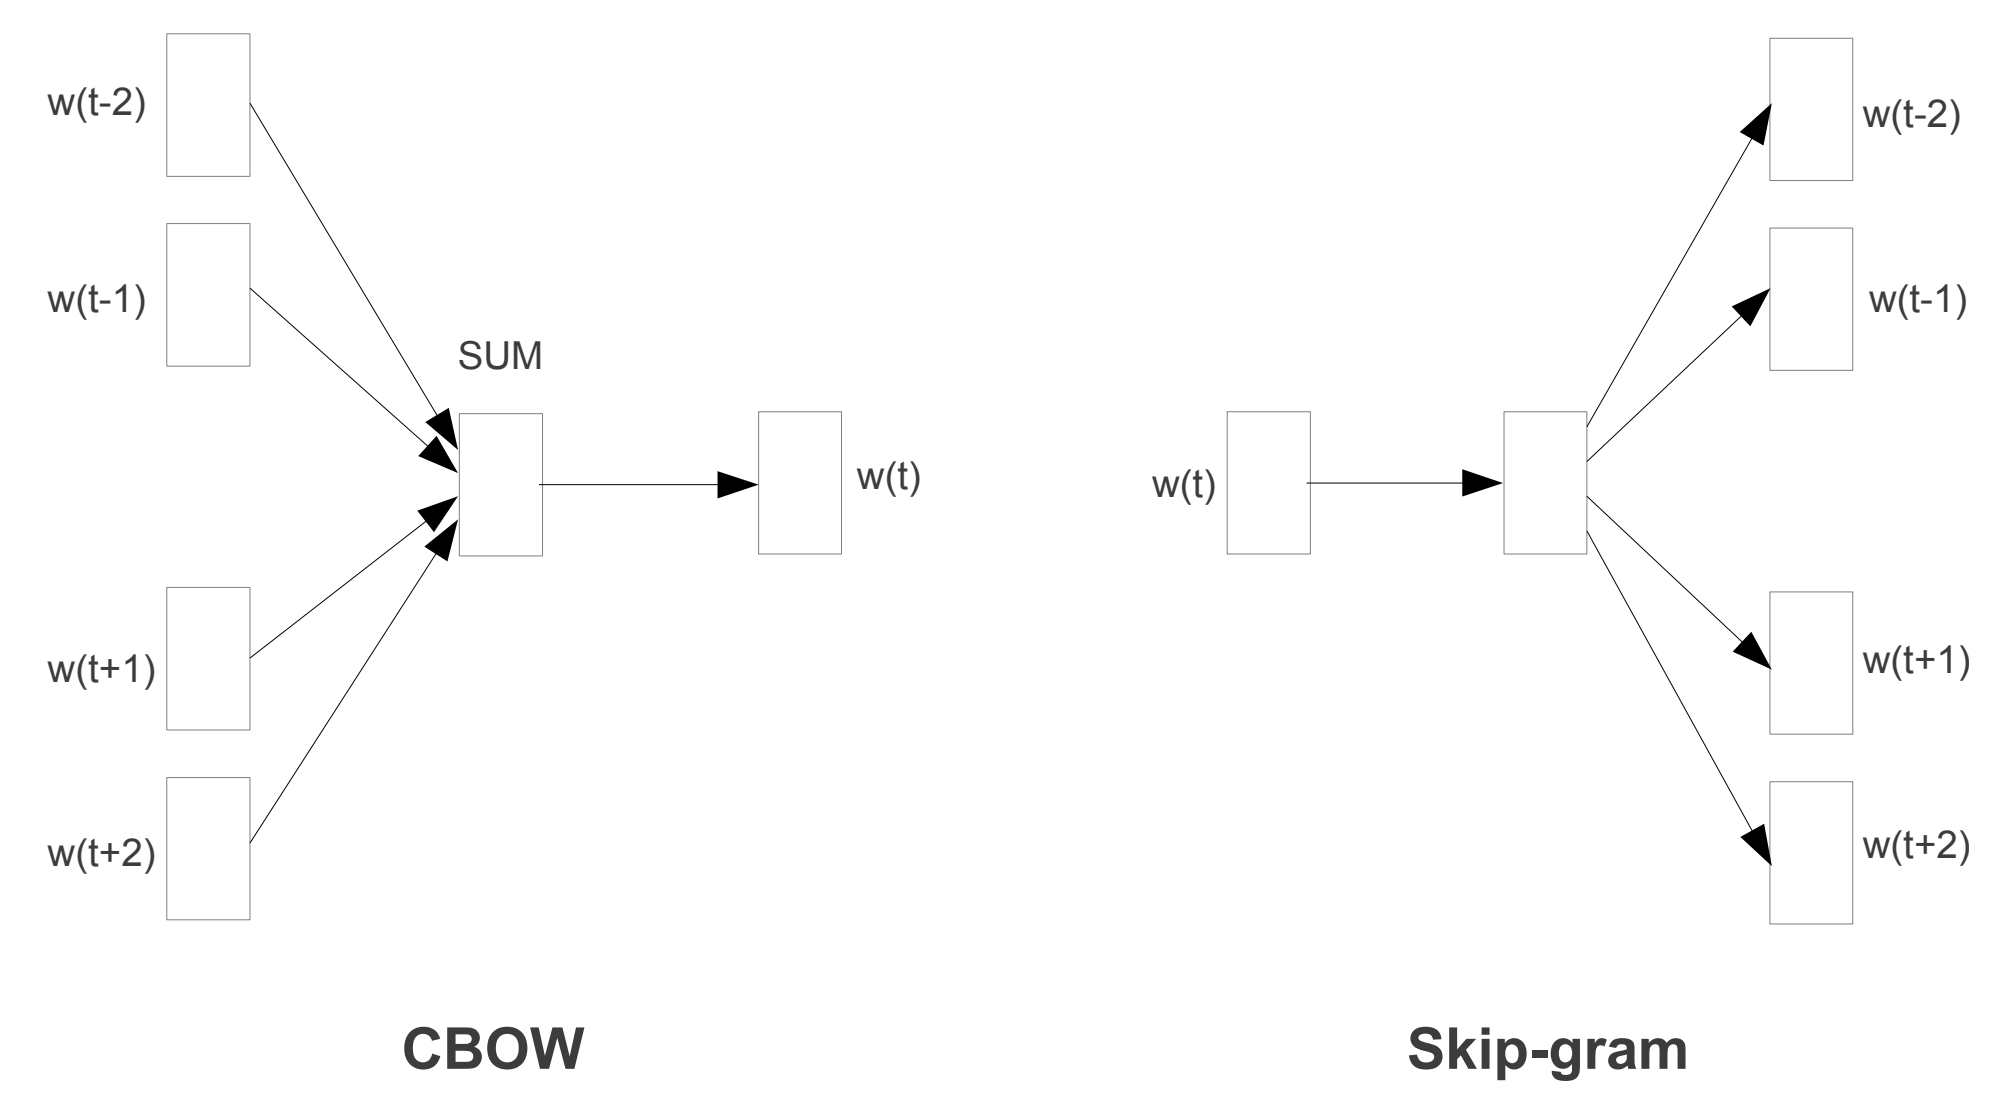
\includegraphics[width=0.7\linewidth]{7_marco_teorico/imagenes/cbow_skipgram.jpg}
	\caption{La arquitectura CBOW predice la palabra actual basado en el contexto, mientras que la arquitectura Skip-gram predice palabras vecinas dada una palabra como entrada \citep{mikolov2013efficient}.}
	\label{fig:cbowskipgram}
\end{figure}

\paragraph{Modelo Skip-Gram}
El modelo Skip-gram se basa en lo siguiente: dado un conjunto de frases (llamado \textit{corpus}) el modelo analiza las palabras de cada sentencia y utiliza cada palabras para predecir las palabras que serán vecinas. La entrada para este modelo es una sola palabra \(w_I\) y la salida, su contexto \(\{w_{0,1},..., w_{0,C}\}\) definido por una ventana de tamaño \(C\). Una potencial instancia de entrenamiento podría ser la palabra “auto” como entrada y las palabras \{"Manejé","mi","hacia","la","tienda"\} las salidas. El objetivo es, mediante el entrenamiento, generar los pesos de la capa oculta de la red neuronal y usarlos como los vectores que representarán las palabras. Mediante la palabra que es usada como entrada, el modelo busca palabras “vecinas” pertenecientes a su contexto y elige una de forma aleatoria. La red neuronal dará como resultado la probabilidad de cada palabra en nuestro vocabulario de ser \textit{palabra vecina}. El concepto de palabra vecina, viene dado por el tamaño de ventana que hayamos elegido, si el tamaño de ventana es 5, significa que son tomadas en cuenta 5 palabras adelante y 5 palabras atrás (10 en total) \citep{skipgrammodel}.

\bigskip La entrada de la red neuronal será una palabra representada como \textit{one-hot vector}, un vector con tantas posiciones como tamaño tenga el vocabulario; esto es, si tenemos un vocabulario de 10000 palabras, el vector tendrá el valor 1 en la posición donde se encuentre la palabra representada, y 0 en las 9999 restantes. La salida de la red neuronal, es otro vector con las mismas 10000 posiciones, que en cada posición contiene las probabilidades de que cada una de las palabras sean vecinas de la palabra representada en la entrada. Las probabilidades son calculadas de la siguiente forma. Dado un one-hot vector \(x\) de tamaño \(V\) (cantidad de palabras del vocabulario) correspondiente a la palabra de entrada, y un conjunto de redes neuronales de la capa oculta de tamaño \(N\). Dado una ventana de tamaño \(C\), tendrémos \(\{y_1,...,y_C\}\) vectores one-hot correspondientes a las palabras de salida en la instancia de entrenamiento. La matriz \(W=V \times N\) es la matriz de pesos entre la capa de entrada y la capa oculta, cuya fila \(i^{th}\) representa los pesos correspondientes a la palabra \(i^{th}\) del vocabulario. Esta matriz \(W\) contiene entonces, la codificación como vector de cada una de las palabras del vocabulario (como filas), las cuales serán entrenadas mediante la red neuronal. El siguiente ejemplo ilustra, cómo la matriz \(W\) multiplicada por el vector de entrada, resulta en el vector que la representa.
\[\begin{bmatrix}0 & 0 & 0 & 1 & 0 \end{bmatrix} \times  \begin{bmatrix}12 & 14 & 2 \\ 6 & 19 & 74 \\ 22 & 33 & 96 \\ 36 & 85 & 2 \\ 95 & 1 & 56 \end{bmatrix} = \begin{bmatrix} 36 & 85 & 2 \end{bmatrix}\]

Se puede ver, cómo el vector resultado de tamaño \(1 \times N\) es la 4 fila de la matriz \(W\), ya que la palabra de entrada es un vector one-hot con el valor \(1\) en el cuarto elemento.

\bigskip Una vez obtenido el vector de salida, éste es usado como entrada para la capa de salida de la red neuronal, usando un clasificador de regresión Softmax \citep{morin2005hierarchical}, el cual es una generalización de la regresión logística para el caso en que se quieren manejar múltiples clases\footnote{Tutorial en profundidad de regresión Softman \url{http://ufldl.stanford.edu/tutorial/supervised/SoftmaxRegression},  Último acceso: Febrero 2021.}. Cada una de las \(V\) neuronas de la capa de salida, producirá un valor entre \(0\) y \(1\). Además, la suma de todos estos valores, será \(1\), es decir, una distribución de probabilidades. Específicamente, cada neurona de salida tiene un vector de pesos correspondiente a cada una de las palabras del vocabulario, que se multiplica con el vector que proviene de la capa oculta y se aplica una función Softmax. El resultado es la probabilidad de que aleatoriamente se seleccione la palabra de entrada y sea vecina a cada una de las palabras representadas por los vectores en las neuronas de salida.

\paragraph{Modelo Continuous Bag of Works (CBOW)}
Es similar al modelo Skip-gram pero con las salidas y las entradas invertidas: dado un conjunto de palabras que definen un contexto, CBOW predice la palabra actual. La capa de entrada consiste en \(C\) palabras del contexto, codificadas como vectores one-hot, es decir un conjunto\( \{x_1,..., x_C\}\) cada uno de dimensión \(V\). La capa oculta es un vector hde tamaño \(N\). Finalmente, la salida es una palabra y también codificada como un vector one-hot. Los vectores de entrada son conectados con la capa oculta por una matriz \(W=V \times N\), y esta capa oculta a su vez es conectada con la capa de salida vía otra matriz \(W'=V \times N\) \citep{cbowmodel}.

\bigskip La salida de la capa oculta \(h\) de la red neuronal es el promedio de los vectores de entrada, ponderados por la matriz \(W\).
\[h = \frac{1}{C}W \cdot (\sum_{i=1}^{C}{x_i})\]
Este cómputo es una de las diferencias principales con el modelo skip-gram. Luego, se calculan las entradas de cada nodo de la capa de salida.
\[u_j = {v'_{w_j}}^{T} \cdot h\]
donde \(v'_{w_j}\) es la \(j^{th}\) columna de la matriz \(W'\). Y finalmente se calcula el resultado de la capa de salida. Dicha salida \(y_j\) es obtenida pasando la entrada \(u_j\) por la función Softmax.
\[y_j=p(w_{y_j}|w_1,...,w_C)=\frac{exp(u_j))}{\sum_{V}^{j=1}exp(u_j')}\]

\subsubsection{FastText}
Fastext\footnote{Sitio de FastText \url{https://fasttext.cc}. Último acceso: Febrero 2021.} es una librería open-source que permite generar representaciones de texto y clasificadores de texto. Está basada en una técnica representación continua de palabras, que tiene en cuenta la morfología\footnote{Parte de la lingüística que estudia las reglas que rigen la flexión, la composición y la derivación de las palabras. Por ejemplo, las distintas conjugaciones de los verbos en español.} de las mismas \citep{bojanowski2017enriching}.
El modelo de FastText está basado en el modelo Skip-gram, donde cada palabra es representada como una bolsa de caracteres \(n-gramas\). Y a cada uno de los n-gramas, se le asignará un vector, que luego, sumados, representarán cada palabra. Dos características muy importantes son, \begin{enumerate*} [label=(\roman*)] \item el método el muy rápido, permitiendo entrenar grandes conjuntos de datos; y \item permite calcular representación de palabras que no aparecen en el conjunto de entrenamiento.  \end{enumerate*}

\bigskip Repasando el modelo skip-gram, introducido por \cite{mikolov2013efficient}, dado un vocabulario \(W\), donde una palabra es identificada por su índice \(w \in \{1,... , W\}\) , el objetivos es aprender la representación vectorial de cada palabra \(w\). Dado un documento grande representado como una secuencia de palabras \(w1, ..., wt\), el objetivo del modelo skip-gram es que las representaciones de la palabras sean entrenadas para predecir bien, otras palabras que aparecen en el contexto, es decir, minimizar la siguiente probabilidad logarítmica:
\[\sum_{t=1}^{T}\sum_{c \in C_t}^{T}{\log p(w_c | w_t)}\]
donde el contexto \(C_t\) es el conjunto de índices de palabras que están alrededor de \(w_t\).

\paragraph{Modelo sub-palabra}
Usando una representación en forma de vector para cada palabra, se ignora la estructura interna de las mismas. El modelo sub-palabra, propone una función de scoring \(s\), con el objetivo de tener en cuenta esta información.
Cada palabra wes representada como una bolsa de n-gramas. Se agregan los símbolos ``\(<\)'' y ``\(>\)'' para delimitar el principio y el final de cada palabra. También, se incluye la palabra en sí misma como otro conjunto de caracteres n-gram. Por ejemplo, la palabra where y con un \(n = 3\) (longitud de la sub-palabras, en este caso sería, tri-gramas), obtenemos:

\begin{center}\ttfamily\sbox{0}{a}%
	\begin{minipage}{45\wd0}% 45 characters here
		\begin{verbatim}
		'<wh', 'whe', 'her', 'ere', 're>' y '<where>'
		\end{verbatim}
	\end{minipage}
\end{center}

Cabe aclarar que los símbolos ``\(<\)'' y ``\(>\)'' también son considerados como caracteres a la hora de construir los n-gramas. Por ejemplo, ``\(<wh\)'' es un trigrama con un delimitador de inicio de palabra.

\bigskip Dado un diccionario de n-gramas de tamaño \(G\) y una palabra \(w\), el set de n-gramas que aparecen en wes \(G_w \in \{1,..., G\}\). Se asocia un vector \(z_g\) a cada n-grama \(g\). Se representa una palabra, como la suma de todas las representaciones vectoriales de sus n-gramas. Entonces, la función scoring, es:
\[s(w,c) = \sum_{g \in G_w}^{}{}z_g^T v_c\]

Este modelo, permite compartir las representaciones entre las palabras y, también, aprender una representación confiable de palabras extrañas o poco frecuentes.

\subsubsection{Semantic Distance}
La \textit{distancia semántica} usada en este trabajo está basada en redes semánticas y estadísticas de corpus \citep{li2006sentence}. El método en cuestión está basado en el cálculo de similaridad entre textos de distancia muy corta, que tiene en cuenta la información semántica y la información del orden de las palabras implicadas en las frases involucradas. La información semántica de las frases es obtenida desde una base de datos léxica y estadísticas de corpus. El uso de una base de datos léxica posibilita modelar el sentido común humano y las estadísticas de corpus adaptar el método a diferentes dominios.

\bigskip Uno de los puntos dominantes por el cual este método es particularmente efectivo para calcular similaridad entre frases cortas se basa en que, tradicionalmente los métodos basados en palabras compartidas funcionan bien solo para textos largos, para los cuales existe una alta posibilidad de que una palabra se encuentre en los documentos en comparación. En cambio, para textos cortos, la coocurrencia de palabras entre ellos es muy rara o nula. Esto se debe a la flexibilidad de los lenguajes de expresar mismos significados usando diferentes frases en términos de estructura y palabras.

\paragraph{El método}
\begin{figure}[h!]
	\centering
	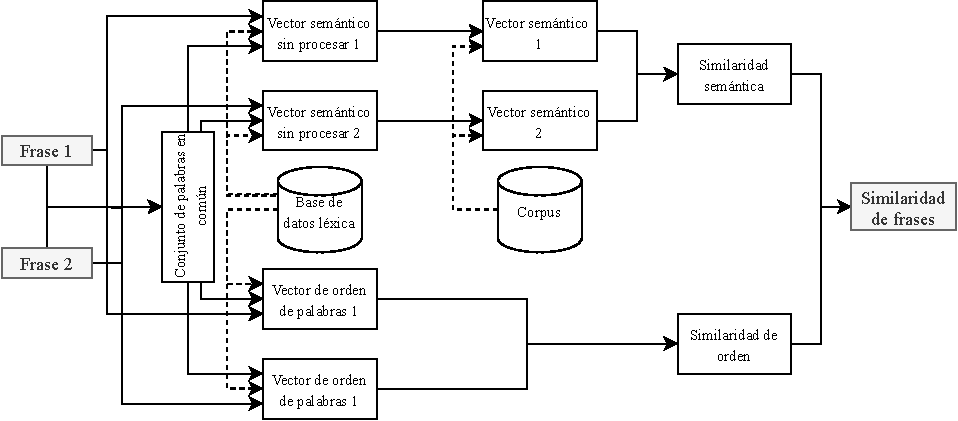
\includegraphics[width=0.9\linewidth]{7_marco_teorico/imagenes/similaridad_sematinca_metodo}
	\caption{Diagrama de cálculo de similaridad semántica.}
	\label{fig:similaridadsematincametodo}
\end{figure}

El procedimiento de cálculo de similaridad entre dos frases, como se muestra en la Figura \ref{fig:similaridadsematincametodo}, utiliza un conjunto de palabras en común usando todas las palabras distintas en el par de frases (en lugar de usar un conjunto fijo como vocabulario). De cada una de las frases, un vector semántico sin procesar es derivado, utilizando la base de datos léxica. También, un vector de orden de palabras es generado a partir de cada frase utilizando la base de datos. Como cada palabra en una frase, contribuye de forma diferente al significado de la misma, la importancia de cada una de ellas es ponderada utilizando información de contenido derivado del corpus. Combinando la información de corpus con los vectores semánticos sin procesar, se obtienen nuevos vectores semánticos los cuales servirán para calcular la \textit{similaridad semántica}. Una \textit{similaridad de orden} es calculada usando los dos vectores de orden previamente generados. Finalmente, la similaridad entre frases es calculada combinando la similaridad semántica y la similaridad de orden.

\paragraph{Similaridad semántica entre palabras}
Las bases de conocimiento tienden a representar el sentido común humano con una estructura jerárquica para un dominio específico o para un lenguaje en general. Existen varios proyectos lingüísticos disponibles en la web, tales como WordNet \citep{miller1995wordnet}, Spatial Date Transfer Standard de la USGS\footnote{United States Geological Survey. https://www.usgs.gov/. Último acceso: Febrero 2021.}, y Gene Ontology\footnote{Gene Ontology. http://geneontology.org/. Último acceso: Febrero 2021.}. Esta estructura jerárquica, se puede modelar como una taxonomía de conceptos.

\bigskip Dadas dos palabras \(w_1\) y \(w_2\), es necesario encontrar la similaridad \(S(w_1,w_2)\) entre ellas. Esto es posible analizando la base de datos léxica (en este caso WordNet si se cuenta con palabras en el idioma inglés) de la siguiente forma: Las palabras están organizadas como conjuntos de sinónimos (llamados \textit{synsets}), con relaciones semánticas a otros synsets. Un método directo para calcular la similaridad es encontrar el camino más corto que conecta dos palabras. Por ejemplo, si tomamos la estructura detallada en la Figura \ref{fig:taxonomiasemantica}, el camino más corto para conectar \textit{niño} y \textit{niña} sería \textit{niño-persona masculina-humano-persona femenina-niña}, y tiene una longitud de \(4\). El synset de personas es llamado \textit{subsumidor mínimo de palabras}, tal como se menciona en la sección \ref{paragraph:similaridad}, ya que sirve de anclaje entre los dos conceptos para los cuales se quiere calcular la distancia semántica.

\begin{figure}[h!]
	\centering
	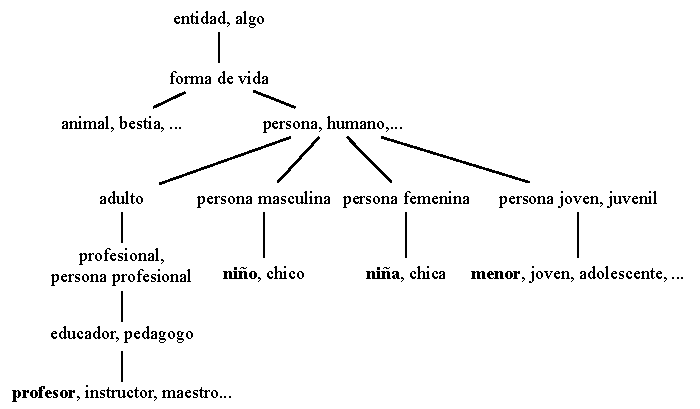
\includegraphics[width=0.9\linewidth]{7_marco_teorico/imagenes/taxonomia_semantica}
	\caption{Base de datos semántica de forma jerárquica.}
	\label{fig:taxonomiasemantica}
\end{figure}

También, se puede ver que la distancia entre \textit{niño} y \textit{profesor} es 6, mientras la distancia entre \textit{niño} y \textit{animal} es 4, lo cual es contraintuitivo e indica que el proceso es mejorable agregando más información de estas estructuras jerárquicas. Es evidente que los synsets pertenecientes a capas altas de la estructura tienen conceptos semánticos más generales y menos similaridad entre ellos y en capas inferiores, sucede lo contrario, conceptos más particulares y similares. Lo anterior sugiere tomar en cuenta la profundidad en jerarquía. Para resumir, la similaridad entre palabras es determinada, no solo por el camino más corto entre ellas, sino también por la profundidad jerárquica, es decir:
\[S(w_1,w_2)=f(l,h)\]

donde \(l\) es el camino más corto entre \(w_1\) y \(w_2\), y \(h\) es la profundidad del subsumer de las mismas en la jerarquía de la red semántica.

\paragraph{Similaridad semántica entre frases}
Contrariamente a métodos clásicos que usan vocabularios con miles de palabras precompiladas, este método semántico usa únicamente vectores semánticos formados por las frases en comparación. Un conjunto de palabras comunes \(T\) es formado por la unión de las dos frases en comparación, luego, un vector semántico léxico es derivado. Cada entrada del vector corresponde a una palabra del conjunto de palabras comunes, lo cual indica que la dimensión del vector es igual al número de palabras del conjunto. El valor de una entrada del vector semántico es calculado de la siguiente forma:
\begin{itemize}
	\item \textbf{Caso 1}.  Si \(w_i\) aparece en la frase, \(s_i\) es 1.
	\item \textbf{Caso 2}. Si \(w_i\)  no está contenida en \(T_1\), una similaridad semántica es calculada entre \(w_1\) y cada palabra en \(T_1\) utilizando el método de la sección anterior.
\end{itemize}

Luego, es necesario ponderar cada una de las palabras basadas en su contenido de información \citep{ribadas2005semantic}. Cada celda es ponderada por la información de contenido \(I(w_i)\) y \(I(\widetilde{w}_i)\). Finalmente, el valor de la entrada del vector semántico es:
\[s_i = \check{s} \cdot I(w_i) \cdot I(\widetilde{w}_i)\]

donde \(w_i\) es una palabra en el conjunto de palabras comunes, y \(I(\widetilde{w}_i)\) es su palabra asociada en la frase. Entonces, la similaridad semántica entre dos frases es definida como el coeficiente del coseno entre los dos vectores:
\[S_s = \frac{s_1.s_2}{||s_1||.||s_2||}\]

\paragraph{Similaridad de orden entre frases}
Consideremos dos frases \(T_1\) y \(T_2\), por ejemplo:
\begin{itemize}
	\item \textbf{T1}:  A quick brown dog jumps over the lazy fox.
	\item \textbf{T2}. A quick brown fox jumps over the lazy dog.
\end{itemize}

Estas frases tienen exactamente las mismas palabras, pero dos de ellas, ubicadas en orden inverso. Como las dos frases contienen las mismas palabras, un método basado en Bag of Words, resultará en que las frases son idénticas, pero para un intérprete humano, es claro que las frases sólo son similares en cierto grado. Por lo cual, un método computacional de similaridad entre frases debe tener en cuenta el orden de las palabras. En el ejemplo, el conjunto de palabras comunes es:

\begin{center}\ttfamily\sbox{0}{a}%
\begin{minipage}{45\wd0}% 45 characters here
	\begin{verbatim}
T = {A quick brown dog jumps over the lazy fox}
	\end{verbatim}
\end{minipage}
\end{center}

Para lograr esto, este método asigna un índice único por cada palabra en \(T_1\) y \(T_2\), en orden, armando un arreglo de palabras. Un vector de orden \(r\) es formado para \(T_1\) y \(T_2\), respectivamente, basado en el conjunto de palabras comunes. Tomando \(T_1\) como ejemplo, por cada palabra \(w_i\) en \(T\), se intenta encontrar la palabra más similar en \(T_1\) de la siguiente forma:
\begin{enumerate}
	\item Si la misma palabra está presente en \(T_1\), la entrada por la palabra en \(r_1\) será el índice de la misma en \(T_1\). Caso contrario, se intenta buscar la palabra más similar \(\widetilde{w}_i \) semánticamente.
	\item Si la similaridad entre \(w_i\) y \(\widetilde{w}_i \) es mayor al umbral, la entrada de \(w_i\) en \(r_1\) es completada con el índice de \(\widetilde{w}_i \) en \(T_1\).
	\item Si las dos búsquedas anteriores fallan, la entrada de \(w_i \) en \(r_1\) es \(0\).
\end{enumerate}
Aplicando este procedimiento a las frases de ejemplo, tenemos:
\[r_1 = \left \{\;1\;2\;3\;4\;5\;6\;7\;8\;9\;\right \}\]
\[r_2 = \left \{\;1\;2\;3\;9\;5\;6\;7\;8\;4\;\right \}\]
Se propone una medida de similaridad de orden entre frases como:
\[S_r = 1 - \frac{\left \| r_1 - r_2 \right \|}{\left \| r_1 + r_2 \right \|}\]
Esto significa que la similaridad de orden de palabras es determinada por la diferencia normalizada del orden de palabras.

\paragraph{Similaridad total entre frases}
La similaridad semántica y la información sintáctica (en términos del orden de las palabras) convergen en el significado de la oración. Entonces, la similaridad total entre frases es definida como la combinación de la similaridad semántica y la similaridad del orden de palabras:
\[S(T_1, T_2)=\delta S_s + (1 - \delta)S_r\]
\[S(T_1, T_2)=\delta \frac{s_1.s.2}{\left \| s_1 \right \|\left \| s_2 \right \|} + (1 - \delta)\frac{\left \|r_1-r_2  \right \|}{\left \| r_1+r_2 \right \|}\]

\bigskip donde \(\delta \leq 1\) decide la contribución relativa de cada una de las medidas de similaridad. Como el orden de palabras cumple un rol subordinado, se recomienda que \(\delta\) tenga un valor mayor a \(0.5\).

